\documentclass[11pt]{article}
% RFP specifically says to use 11 point type and 1 inch margins
\usepackage{graphicx}
\usepackage{epsf,color}
\textwidth=6.5in\oddsidemargin=0in \evensidemargin=0in \topmargin
0pt \advance \topmargin by -\headheight \advance \topmargin by
-\headsep \textheight 9.0in

%\textwidth=6.5in\oddsidemargin=0in \evensidemargin=0in \topmargin
%0pt \advance \topmargin by -\headheight \advance \topmargin by
%-\headsep \textheight 8.9in

\usepackage{amsmath}
\usepackage{graphicx}
\usepackage{dcolumn}
\usepackage{multirow}
\usepackage{wrapfig}
\usepackage[compact]{titlesec}

%\usepackage[plain]{fullpage}
\usepackage{amsfonts}
%\usepackage{lastpage}
%\usepackage{fancyhdr}

\usepackage[version=3]{mhchem} 
% you can use this command to skip chunks of your document
% just put the command around the chunk like this
% \comment{ ...the chunk... }
\newcommand{\comment}[1]{}

%\newcommand{\MarginPar}[1]{\hspace{1sp}\marginpar{\tiny\sffamily\raggedright\hspace{1sp}#1}}
\setlength{\marginparwidth}{0.75in}
\newcommand{\MarginPar}[1]{\marginpar{%
\vskip-\baselineskip %raise the marginpar a bit
\raggedright\tiny\sffamily
\hrule\smallskip{\color{red}#1}\par\smallskip\hrule}}

\definecolor{drkgrn}{rgb}{0.043,0.341,0.2274}
\newcommand{\remrg}[1]{ {\it \color{drkgrn} \{#1 -RG\}}}

%\renewcommand{\baselinestretch}{1.05} % = 1.0 Single space; = 2.0 Double
\renewcommand{\baselinestretch}{1.0} % = 1.0 Single space; = 2.0 Double

%\renewcommand{\refname}{Literature Cited}
%------------------------

%\pagestyle{empty}  % No page numbers
%\textfloatsep 0mm
%\abovecaptionskip 1mm

\begin{document}

%\pagestyle{plain}
%\pagenumbering{roman}
\begin{center}
{\Large{\textbf{Point defect formation kinetics}}}
\end{center}

 
\subsection*{Point defect formation in thin-film photovoltaics:}
A key design need for high efficiency photovoltaic devices based on
newer materials is the ability to control intrinsic point defect
formation to achieve effective n+ and p+ doping. Unlike traditional
(e.g., $Si$) materials where dopant atoms are purposefully introduced,
these newer materials (such as CZTS) are self doped by intrinsic
defects including vacancies, antisite and interstitial defects
\cite{JiangY13}.

{\it First principles calculations have suggested that there is a
  theoretical configuration for such materials as CZTS and CIGS that
  leads to a combination of carrier concentrations, mobility and
  minority carrier lifetime that would provide exceptional device
  performance. However, the question of how to control process
  conditions during film deposition to arrive at such a configuration
  remains open. Modelling the kinetics of point defect formation
  through pseudo-reactions results in a system of differential
  equations that are tightly coupled and indicate the resulting
  properties have a non-trivial relationship to the intrinsic
  defects.  Electronic structure calculations can provide an estimate
  fo the energy difference when defects are formed but the kinetic
  parameters (energy barriers) are the result of indirect measurements.}

For example, an abstract metal-sulfide system could be described by a
simplistic system of four reactions expressing an oxidation reaction,
the Schottky disorder and creation of anion vacancies. Systems of
practical interest (e.g., CZTS, CIGS, etc.) are far more complicated
and involve 10s-100s of possible defect formation relations.

\begin{eqnarray*}
\ce{ \tfrac{1}{2} S2 -> S_s^x + V_m^{''} + 2 h^+ } \\
\ce{ NULL -> V_m^{''}+ V_s^{$\cdot \cdot$} } \\
\ce{ NULL -> e^' + h^{$\cdot$} } \\
\ce{ S_s^x -> \tfrac{1}{2} S2 + V_s^{$\cdot \cdot$} + 2 e^- }.
\end{eqnarray*}

Where the rate of the $\alpha^{\mathrm{th}}$ reaction is approximated
by the Arrhenius form:
\begin{equation}
  \label{eq:1}
  k_\alpha e^{-(E_a)_\alpha/(RT)}
\end{equation}

There is also a transport component here: diffusion of the non-metal
species ($S_2$ above) into the film can be included and may be
rate-limiting. Even in the 0-D case, for the M-S example system, the
ambient $S_2$ partial pressure is a key parameter that when varied
results in equilibrium states with different doping (performance)
characteristics.  Time-dependent histories of the external conditions
during crystal growth can be expected to access quasi-equilibrium
states. Many of these quasi-stable may exist and can have desirable
properties. By varying process conditions, different pathways through
the state space can be generated that may lead to one of many
different quasi-equilibrium conditions. It is desirable from a
development perspective to be able to computationally search for
processing conditions (ambient metal pressure, temperature temporal
variations) that lead to favorable configurations, but to do so the
many parameters appear in the model equations must be refined. 

Direct measurement of the concentration of arbitrary point defects is
difficult and must be inferred from more easily observed
characteristics, leading a model for the observation process $h(x)$
that may be quite complicated and the result of a non-trivial
simulation.  For example, majority carrier concentration, electron or
hole mobility, capacitance can be measured, but these are all
indicators of the final point defect configuration that results from
the process rather than measures of the individual formation
rates. With significantly more effort, the dependence of the film
conductivity on temperature provides an indirect measure of the
activation energy for carrier concentration: this is related to the
kinetic parmeters of the governing defect concentration(s).  A variety
of simulation/experiment pairs are desirable to increase sensitivity
to the various parameters separately:

\begin{itemize}
\item Equilibrium concentrations in an homogenous (0-D) configuration
  are insensitive to the kinetic parmeters and useful to focus
  on the enthalpy differences across the pseudo-reactions. 
\item Alternatively, a time-dependent solution can be sought. This
  adds complexity to the model and input parameters: it requires
  kinetic rates as inputs but can also handle time-dependent boundary
  conditions and arrive a quasi-equilibrium states depending on the
  initial conditions. These experiments are useful to to emphasize the
kinetic parameters (energy barriers). 
\item Finally, adding increasing spatial dimension, i.e., normal to
  the surface allows concentration gradients to be captured and the
  comparison to focus also on transport properties. 
\end{itemize}

While the solution of the multi-dimensional problem involves the
influence from all of the parameters under consideration, alone it is
is less selective to the individual parameters. By performing a
collection of experiments emphasizing the different aspects of the
problem we can improve distinguishability to build up our improved
estimates of the inputs. 

\begin{figure}[h]
  \centering
  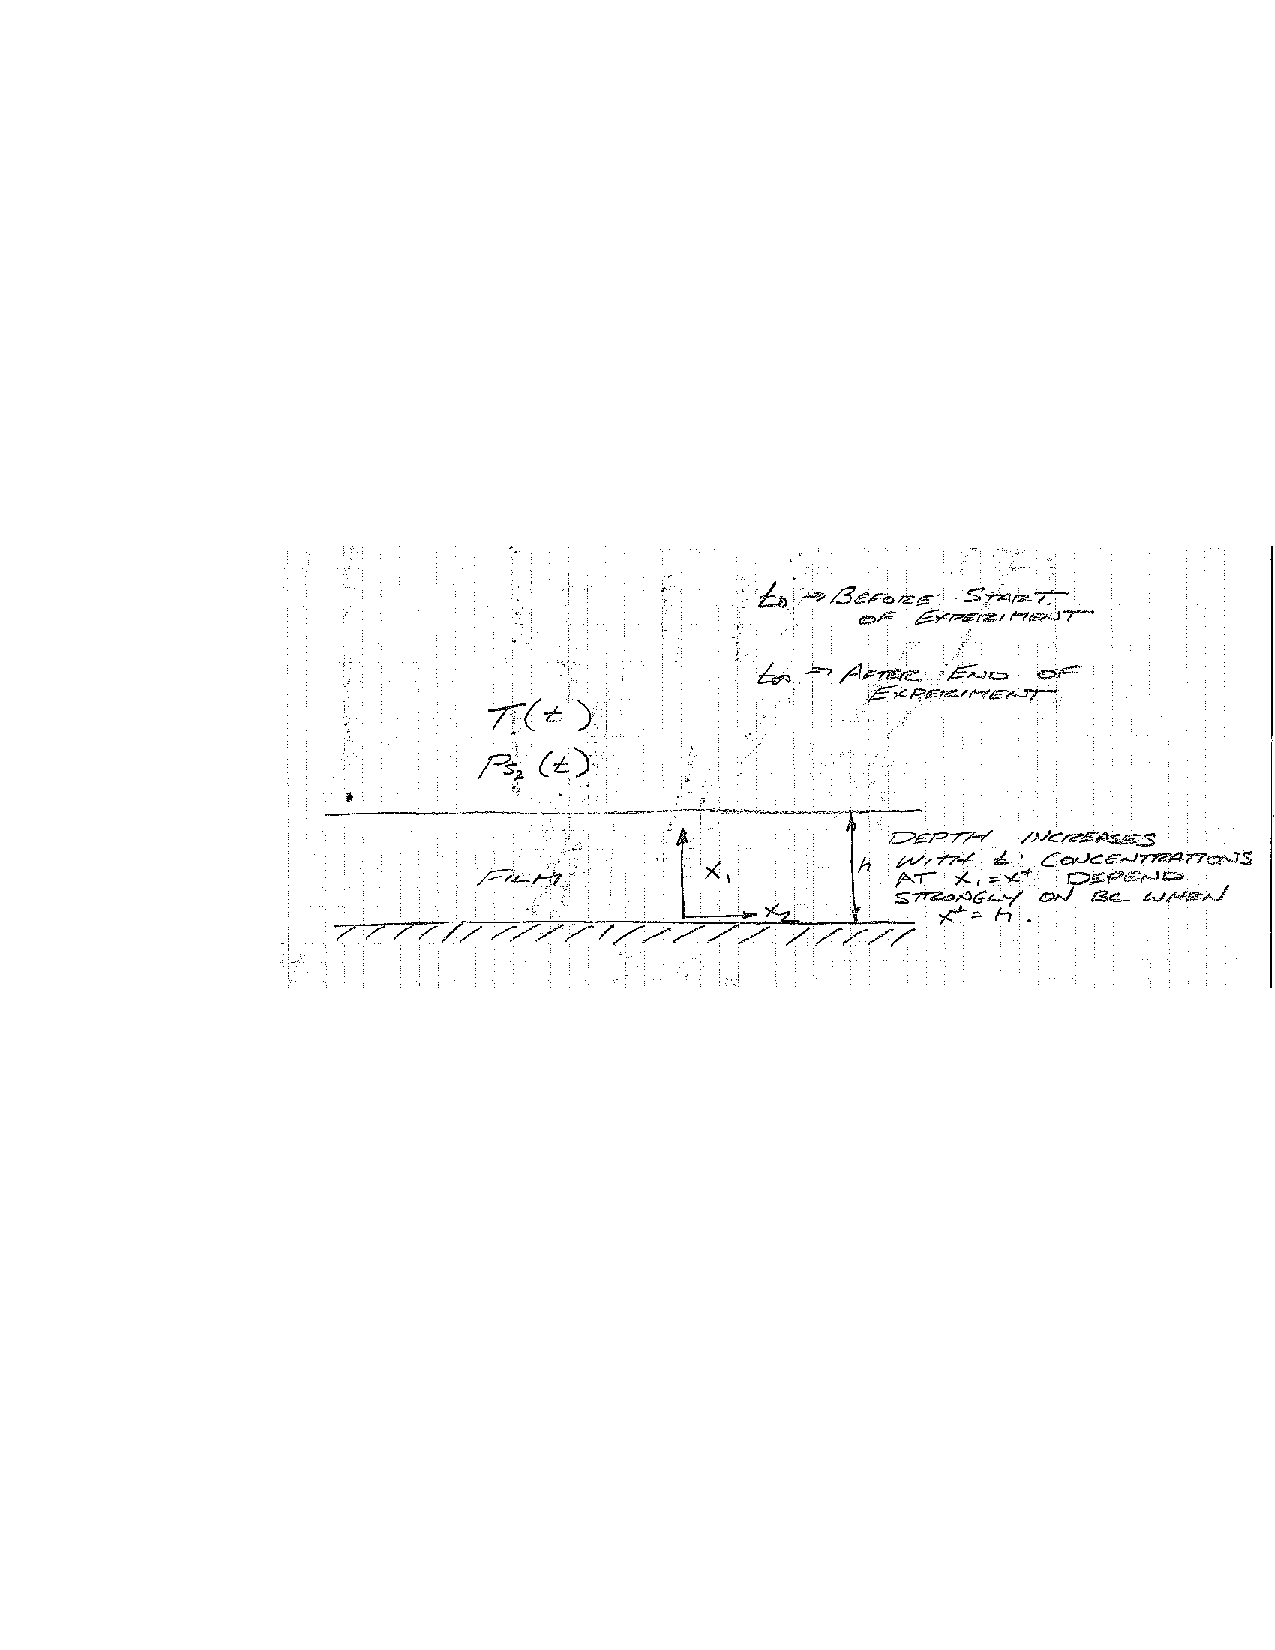
\includegraphics[width=0.8\textwidth]{pd_sketch.pdf}
  \caption{Sketch of film deposition}
  \label{fig:film}
\end{figure}


\remrg{The experimental process parameters could be
  thought of as either an uncertain input, albeit not one we're
  trying to constrain, or as an observable. At first glance the latter
  seems more appropriate.}

%\begin{table}[h]
%  \centering
%  \begin{tabular}{l l l l l}
%    Level in hierarchy & Model inputs & Observables & Processes
%    addressed \\
%    \hline
%    0-D, steady & $(E_a)_\alpha$  & $p_{S_2}(t_0)$ & Equilibrium
%    concentrations \\
%    & & $T(t_0)$ & \\
%    & & $h^+(t_\infty)$ & \\
%    & & $e^-(t_\infty)$ & \\
%    \hline
%    0-D, unsteady & $(E_a)_\alpha$& $p_{S_2}(t)$ & Time dependent
%    bcs \\
%    & $k_\alpha$ & $T(t)$ & Quasi-equilibrium states \\
%    & & $h^+(t_\infty)$ & Dependence on ICs \\
%    & & $e^-(t_\infty)$ & \\
%
%    \hline
%    1-D, unsteady & $(E_a)_\alpha$& $p_{S_2}(t)$ & Time dependent
%    bcs \\
%    & $k_\alpha$ & $T(t)$ & Quasi-equilibrium states \\
%     & $D_j$ &$h^+(t_\infty)$ &  Dependence on ICs \\
%     & & $e^-(t_\infty)$ & Finite rate transport \\
%     & && Time dependent bcs coupled \\
%     & & &    to finite rate transport \\
%  \end{tabular}
%  \caption{Inputs, observables and physical processes included in
%    possible PD simulation hierarchy. }
%  \label{tab:pdh}
%\end{table}


\bibliographystyle{plain}

\bibliography{pd.bib} 



\end{document}
